\documentclass[tikz,border=8pt]{standalone}
% Shared look for every TikZ diagram. Load with \input{../../tools/tikz-style.tex}
\usepackage[T1]{fontenc}
\usepackage{lmodern}
\renewcommand{\sfdefault}{lmr}  % diagrams use the same serif as the text
\usetikzlibrary{arrows.meta, positioning, shapes.geometric, calc, fit, backgrounds}
\definecolor{cblue}{HTML}{4C78A8}
\definecolor{corange}{HTML}{F58518}
\definecolor{cgreen}{HTML}{54A24B}
\definecolor{cred}{HTML}{E45756}
\definecolor{cpurple}{HTML}{B279A2}
\definecolor{cgrey}{HTML}{6B6B6B}
\tikzset{
  every picture/.style={font=\sffamily, line width=1.2pt},
  box/.style={draw=#1, fill=#1!12, rounded corners=4pt, align=center, inner sep=7pt, minimum height=1.1cm},
  box/.default=cgrey,
  arrow/.style={-{Stealth[length=3mm]}, draw=cgrey, line width=1.4pt},
  title/.style={font=\sffamily\bfseries\Large},
  note/.style={font=\sffamily\small, text=cgrey, align=center},
}
\AtBeginDocument{\hyphenpenalty=10000 \exhyphenpenalty=10000}

\begin{document}
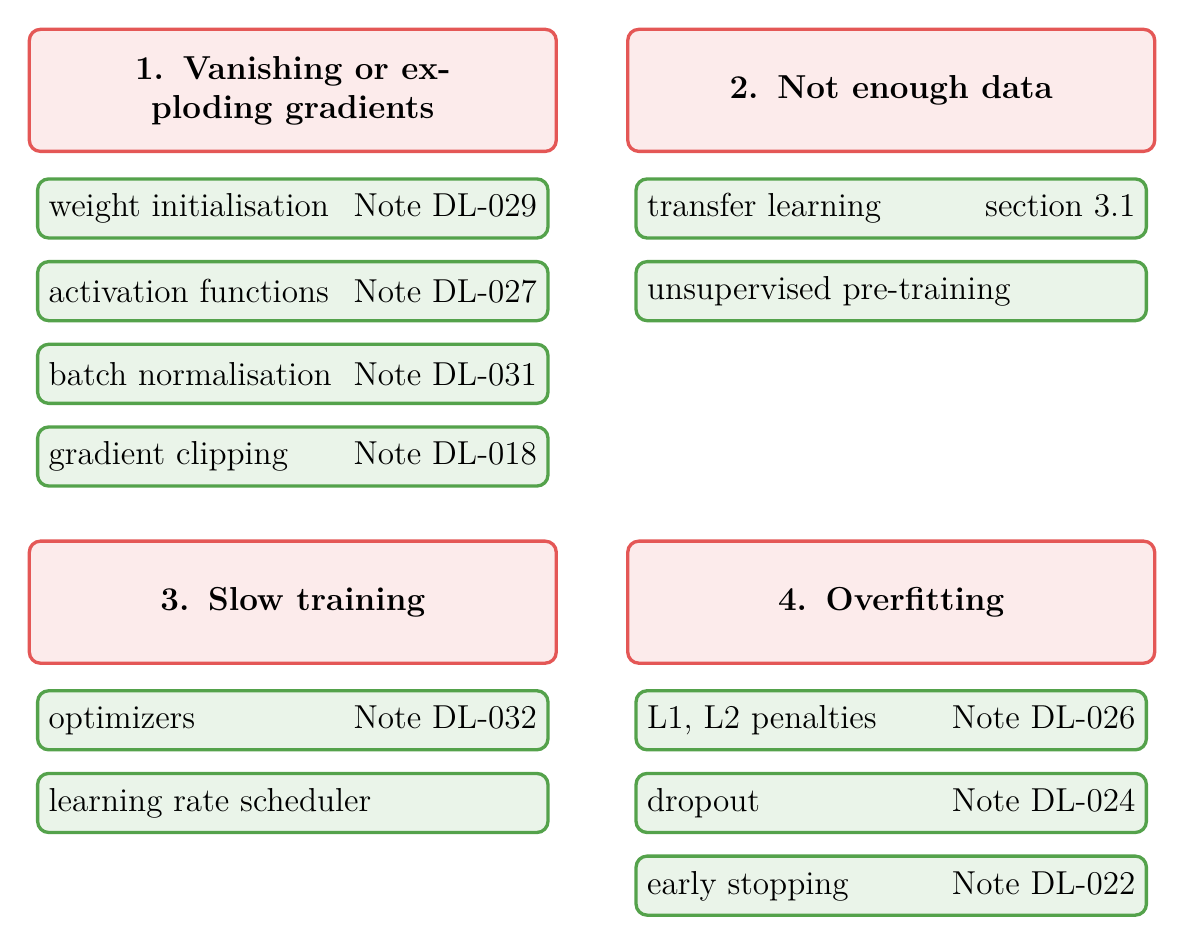
\begin{tikzpicture}[every node/.append style={font=\sffamily\large},
  prob/.style={box=cred, text width=6.2cm, font=\sffamily\bfseries\large, minimum height=1.55cm},
  chip/.style={box=cgreen, text width=6.2cm, minimum height=0.75cm, inner sep=4pt, align=left}]
  \foreach \X/\Y/\p/\list in {
     0/0/{1. Vanishing or exploding gradients}/{weight initialisation{\hfill}Note DL-029, activation functions{\hfill}Note DL-027, batch normalisation{\hfill}Note DL-031, gradient clipping{\hfill}Note DL-018},
     7.6/0/{2. Not enough data}/{transfer learning{\hfill}section 3.1, unsupervised pre-training},
     0/-6.5/{3. Slow training}/{optimizers{\hfill}Note DL-032, learning rate scheduler},
     7.6/-6.5/{4. Overfitting}/{{L1, L2 penalties{\hfill}Note DL-026}, dropout{\hfill}Note DL-024, early stopping{\hfill}Note DL-022}} {
    \node[prob] (h) at (\X,\Y) {\p};
    \foreach \c [count=\k] in \list {
      \node[chip] at (\X, \Y-0.45-1.05*\k) {\c};
    }
  }
\end{tikzpicture}
\end{document}
